\chapter{Computer Networks and the Internet (1-78)}


\lecture{1-5}{19 Feb. 08:00}{First Lecture}

\section{What Is the Internet}

\begin{definition}[public internet]\label{def:public_internet}
    Specific computer network, a system that connects two or more computing devices to transmit and share information.
\end{definition}

\begin{definition}[computing device]\label{def:computing_device}
    A functional unit that can perform substantial computations, including numerous arithmetic operations and logic operations without human intervention. A computing device can consist of a standalone unit or several interconnected units. It can also be a device that provides a specific set of functions, such as a phone or a personal organizer, or more general functions such as a laptop or desktop computer. 
\end{definition}

\begin{definition*}
    The internet can be defined in two ways.
\begin{definition}[nuts and bolts]\label{def:internet1}
    Basic hardware and software components that make up the Internet.
  \end{definition}
  \begin{definition}[networking infrastructure]\label{def:internet2}
     Networking infrastructure that provides services to distributed applications. 
     The hardware and software that enable network connectivity and communication between users, devices, apps, the internet, and more.
  \end{definition}
\end{definition*}
\newpage

    \subsection{A nuts-and-Bolts Description}
        \begin{definition}[Computer network]\label{def:computer_network}
            Interconnects billions of computing devices throughout the world\footnote{Since even devices different than computers are hooked to the Internet this term can be considered outdated}.    
        \end{definition}

\vspace{24pt}

        End systems are connected by communication links and packet switches.

\vspace{12pt}

        The transmission rate of a link is measured in bits/second

\vspace{24pt}

\begin{figure}[h!]
    \centering
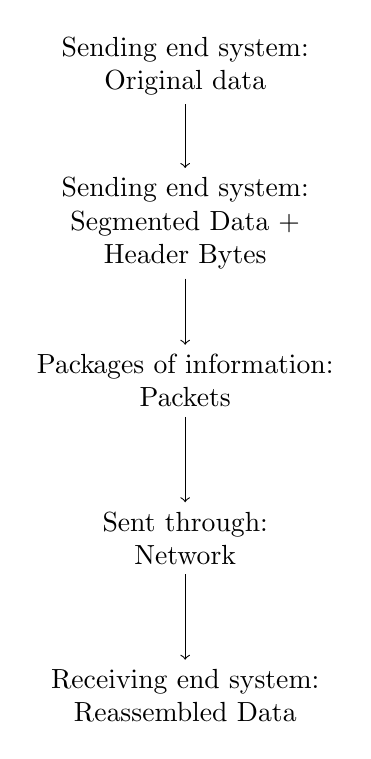
\begin{tikzpicture}[node distance=2cm, auto]

  % Nodes
  \node (data) [align=center] {Sending end system:\\ Original data};
  \node (segment) [below of=data, align=center] {Sending end system:\\ Segmented Data +\\Header Bytes};
  \node (packets) [below of=segment, align=center] {Packages of information:\\ Packets};
  \node (network) [below of=packets, align=center] {Sent through:\\ Network};
  \node (reassembled) [below of=network, align=center] {Receiving end system:\\ Reassembled Data};

  % Arrows
  \draw[->] (data) -- (segment);
  \draw[->] (segment) -- (packets);
  \draw[->] (packets) -- (network);
  \draw[->] (network) -- (reassembled);

\end{tikzpicture}
\caption{Data transmission process in a computer network}\label{fig:data_transmission}
\end{figure}


\vspace{24pt}

\begin{definition*}
    Two main types of packet switches. They forward packets to their ultimate destination
        \begin{definition}[Routers]\label{def:routers}
           Used in network core 
        \end{definition}
        \begin{definition}[Link-layer switches]\label{def:link_layer_switches}
            used in access networks
        \end{definition}
\end{definition*}

\begin{definition}[route or path]\label{def:route_path}
    The path a packet takes from sender to receiver through communication links and switches.    
\end{definition}






\newpage


\lecture{6-24}{9 Sep. 08:00}{Third Lecture}


